
\documentclass{beamer}

% Theme choice:
\usetheme{CambridgeUS}

% Title page details: 

\usepackage{polynom}
\usepackage{amssymb}
\usepackage{amsmath}

\usepackage{bm}
\usepackage[misc]{ifsym}

\usepackage{enumitem}
\usepackage{mathtools}
\usepackage[applemac]{inputenc}
\usepackage{tikz}

\usepackage{parskip}

\DeclareMathOperator*{\Res}{Res}
\DeclareMathOperator*{\equals}{=}
\DeclareMathOperator*{\pipe}{|}

\hyphenation{op-tical net-works semi-conduc-tor}
\def\inputGnumericTable{}  
\graphicspath{{./images/}}


\begin{document}
\newcommand{\bfr}[2]{\section{#1} \begin{frame}{#1} #2 \end{frame}}

	\title{Assignment 10}
		\author{ Abhay Shankar K: CS21BTECH11001}
\date{}
	\begin{frame}
    		\titlepage
	\end{frame}

	\begin{frame}{Outline}
    		\tableofcontents
	\end{frame}

	\providecommand{\brak}[1]{\ensuremath{\left(#1\right)}}
	\providecommand{\mn}[2]{\ensuremath{min\brak{#1, #2}}}
	\providecommand{\mx}[2]{\ensuremath{max\brak{#1, #2}}}
	\providecommand{\rpr}[2]{\ensuremath{P_{#1}\left(#2\right)}} %random variable notation
	\providecommand{\spr}[1]{\ensuremath{P\left(#1\right)}} %simple notation
	\newcommand{\abs}[1]{\left| #1 \right|}
	
	\providecommand{\pmf}[2]{\ensuremath{f_{#2}\left(#1\right)}}
	\providecommand{\cdf}[2]{\ensuremath{F_{#2}\left(#1\right)}}
	
	\bfr{Question}{
		Let $X$ and $Y$ be two independent random variables with common pmf :
		\begin{align}
			\rpr{X}{k} &= pq^k\ \text{where}\ q = p - 1\nonumber \\
			&\forall \brak{k \geq 0} \in \mathrm{Z} 
				\label{pmf}
		\end{align}
		
		Show that the following pairs of RV's are independent.
		\begin{enumerate}[label = \brak{\textbf{\roman*}}]
			\item $\mn{X}{Y}$ and $X - Y$.
			\item $Z = \mn{X}{Y}$ and $W = \mx{X}{Y} - \mn{X}{Y}$
		\end{enumerate}
	}
	
	\bfr{Solving for $p$}{
		Due to unitarity,
		\begin{align}
			\Sigma_{k = 0}^{\infty} \rpr{X}{k} &= 1 \nonumber \\
			\implies \Sigma_{k = 0}^{\infty} p\brak{p - 1}^k &= 1 \nonumber \\
			\implies \frac{p}{2 - p} &= 1 \nonumber \\
			\implies p = 1
				\label{p}
		\end{align}

		Therefore, the PMF becomes a Kronecker Delta function, $\rpr{X}{k} = \delta \brak{k}$. 
		We shall be leveraging several of the properties of the delta function for the solution.
	}

	\bfr{Solution:}{
		\begin{block}{\brak{\textbf{\textrm{i}}}}
			Clearly,
			\begin{align}
				\spr{Z = k \; \& \; \brak{X - Y} = k} &= \delta\brak{k}
			\end{align}
			And also,
			\begin{align}
				\rpr{Z}{k} \times \spr{\brak{X - Y} = k} &= \delta\brak{k} \times \delta\brak{k} \nonumber \\
				&= \delta\brak{k}
			\end{align}
			$\therefore Z = \mn{X}{Y}$ and $X - Y$ are independent.
			
		\end{block}
	}

	\bfr{}{
		\begin{block}{\brak{\textbf{\textrm{ii}}}}
			Clearly,
			\begin{align}
				\spr{Z = k \; \& \; W = k} &= \delta\brak{k}\\
			\end{align}
			And also,
			\begin{align}
				\rpr{Z}{k}\times \rpr{W}{k} &= \delta\brak{k} \times \delta\brak{k} \nonumber \\
				&= \delta\brak{k}
			\end{align}
			$\therefore Z = \mn{X}{Y}$ and $W = \mx{X}{Y} - \mn{X}{Y}$ are independent.
			
		\end{block}
	}

	\bfr{Graph}{
		\begin{figure}[h!]
			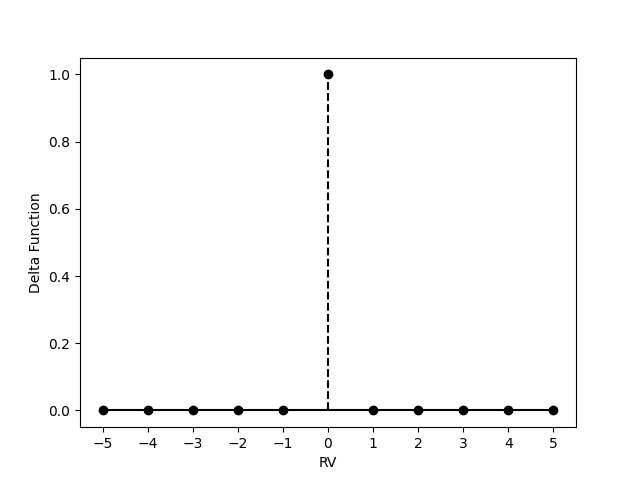
\includegraphics[scale = 0.4]{assig10_del.png}
		\end{figure}
	}
	
								
\end{document}
	
	

	
	
	
	